%%% Local Variables:
%%% mode: latex
%%% TeX-master: "../index"
%%% End:

% Recommended:
% Complexity of collisions (preimage)
% - Birthday paradox
% How to build hash functions
% - Blocks with padding
% - Merkle-Damgaard
% - Why is it secure?

\subsection*{Agenda}
\begin{enumerate}
\item Properties of hash-functions
\item Complexity of collisions
\item Iterated Hash-functions
\item Merkle-Damgård construction
\end{enumerate}

\subsection{Properties of Hash functions}
\textbf{Hash functions} takes a input of a binary string of arbitrary
length and returns a binary string of fixed length.
\begin{figure}[H]
  \centering
  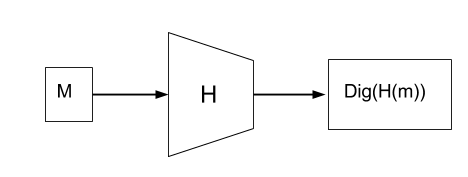
\includegraphics[scale=0.4]{images/10-hash}
  \caption{Model for hashing a message}
\end{figure}

\textbf{The ideal Hash function} has 4 main properties:
\begin{itemize}
\item It is easy to compute the hash value for any given message
\item It is infeasible to generate a message that has a given hash (pre-image)
\item It is infeasible to modify a message without changing the hash
\item It is infeasible to find two different messages with the same hash (collision)
\end{itemize}

\textbf{Security of Hash functions}

% \textbf{Private key:}

% \textbf{Private key:}

\subsection{Complexity of collisions}
\subsubsection*{Birthday paradox}
Probability of finding a collision. Given a function $f$ that maps
values to $H$ different outputs, the probability of finding a
collision after $n$ randomly selected inputs is

\[ p(n; H) \approx 1 - e^{\frac{-n(n-1)}{2H}} \approx 1 - e^{\frac{-n^2}{2H}} \]

This expression can be invertedto $n(p; H)$ describing how many tries
$n$ it takes to reach a probability $p$ of collision

\[ n(p; H) \approx \sqrt{2H \ln \frac{1}{1 - p}} \]

To achieve $0.5$ chance of collision this gives

\[ n(0.5; H) = 1.1774 \sqrt{H} \]

\textbf{Example:} For a 128 bit hash there are $2^{128}$ different
hashes, and the number of tries needed to achieve $0.5$ chance of
collision is then

\[ 1.1774 \sqrt{2^{128}} \approx 2.17 \cdot 10^{19} \]

\subsection{Iterated Hash-functions}
\begin{itemize}
\item Hash-function must be able to process an arbitrary-length
  message into a fixed-length output.
\item Can be achieved by breaking the input up into a series of
  equal-sized blocks, and operating on them in sequence using a
  one-way compression function
\item To make sure the message fits the blocks of the compression
  function, we apply a padding function.
\item We will show that this provides a method for showing that if one
  finds a collision for the hashing function, one also found a
  collision for the compression function.
\end{itemize}

\begin{figure}[H]
  \begin{centering}
    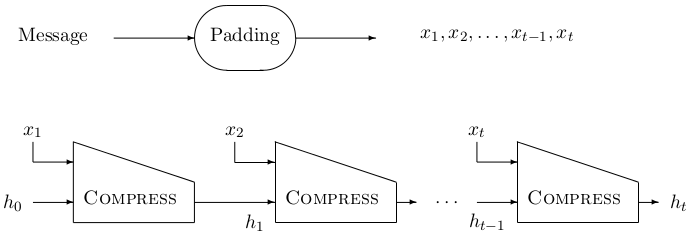
\includegraphics[width=12cm]{images/10-it-hash}
    \caption{Model of iterated hash-functions}
  \end{centering}
\end{figure}

% \begin{figure}[H]
%   \centering
%   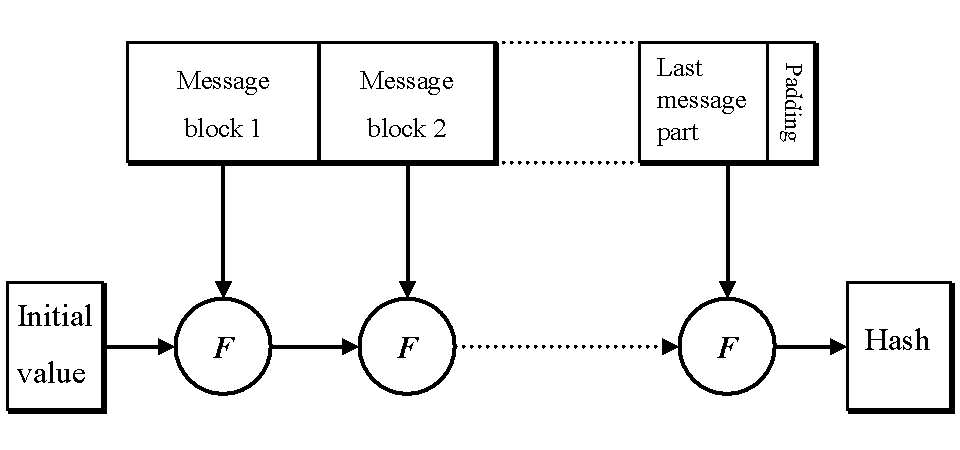
\includegraphics[scale=0.3]{images/10-padding}
%   \caption{Model for hashing using padding}
% \end{figure}

\subsection{The Merkle-Damgård Construction}
Let $h$ be a compression function:
\[ h: \{0,1\}^N \rightarrow \{0,1\}^n \quad \text{where } N > n \]

We construct a hash-function $H$, for some large value $M$:
\[ H: \{0,1\}^M \rightarrow \{0,1\}^n \]

Typical values of $M$ can be $2^{64}-1$ or $2^{128}-1$.

\subsubsection*{Padding}
Begin by computing $l_M$ such that it is the smallest possible where
it holds that $2^{l_M} -1 \ge M$.
\begin{itemize}
\item Let $x \in \{0,1\}^v$ be a $v$-bit string to be hashed
\item First append a one-bit to $x$, that is, $x := x | ‘1’$. Now the length of $x$ is $v + 1$.
\item Let $s$ be the least positive integer such that $v + 1 + s +
  l_M$ is a multiple of $N - n$,\\ e.i. $s \equiv - (v + 1 + l_M) \mod
  (N-n)$
\item Append $s$ zero-bits to $x$.
\item Append to $x$ a block of $l-M$ bits which contains the binary representation of the integer
\end{itemize}

\subsubsection*{Collision}
A hash function built with the Merkle–Damgård construction is as
resistant to collisions as is its compression function; any collision
for the full hash function can be traced back to a collision in the
compression function.

\textbf{Proof}\\
Let $IV \in {0, 1}^n$ be a fixed, randomly chosen value. Let $h$ and $H$ be as above.

Assume there is a collision for $H$. We want to show that then there
is also a collision for $h$ somewhere. Thus, we have two distinct
strings $x \not= x'$, such that $H(x) = H(x')$.

Let $z$ and $z'$ be
the results of padding $x$ and $x'$ according to above rule. Then $z =
z'$.
\begin{align*}
  z = (z_1 , z_2 , \ldots , z_t) \\
  z' = (z'_1 , z'_2 , \ldots , z'_s )
\end{align*}
We will assume that the message lengths that are appended in the
padding rule are (fully) contained in the last blocks, $z_t$ and
$z'_s$.

\textbf{Assume first that $t = s$} \\
We therefore have
\[ H(x) = H(x') \Rightarrow h(h_{t-1} , z_t) = h(h'_{s-1} , z'_s) \]
which gives a collision for $h$, since $z_t$ contains a binary representation
of $t$ and $z'_s$ contains a binary representation of $s$ and $t = s$.

\textbf{Assume next that $t = s$} \\
We now have
\[ H(x) = H(x') \Rightarrow h(h_{t-1} , z_t) = h(h'_{t-1}, z'_t) \]
which gives a collision for $h$, or it holds that
\[ (h_{t-1} , z_t) = (h'_{t-1} , z'_t) \]
In the latter case, this means that
\[ h_{t-1} = h'_{t-1} \Rightarrow h(h_{t-2} , z_{t-1}) = h(h'_{t-2} , z'_{t-1}) \]
Thus, either there is a collision for $h$, or it holds that
\[ (h_{t-2} , z_{t-1}) = (h'_{t-2} , z'_{t-1}) \]

Continuing in this fashion, one finds either a collision for $h$ or it
holds that
\[ z_{t-i} = z_{t-i}\ , \quad  i = 0 \ldots t-1 \]

The latter cannot be true since it was assumed that $z = z'$.
